\documentclass[14pt]{beamer}
\usetheme{Dresden}
\usecolortheme{beaver}

\usepackage{xcolor}
\usepackage{listings}
\usepackage{courier}
\usepackage{graphicx}
\usepackage{amsmath}
\usepackage{algorithm2e}

\definecolor{mGreen}{rgb}{0,0.6,0}
\definecolor{mGray}{rgb}{0.5,0.5,0.5}
\definecolor{mPurple}{rgb}{0.8,0,0.82}
\definecolor{backgroundColour}{rgb}{0.95,0.95,0.92}

\lstdefinestyle{CStyle}{
    backgroundcolor=\color{backgroundColour},   
    commentstyle=\color{mGreen},
    keywordstyle=\color{magenta},
    numberstyle=\tiny\color{mGray},
    stringstyle=\color{mPurple},
    basicstyle=\footnotesize,
    breakatwhitespace=false,         
    breaklines=true,                 
    captionpos=b,                    
    keepspaces=true,                 
    numbers=left,                    
    numbersep=5pt,                  
    showspaces=false,                
    showstringspaces=false,
    showtabs=false,                  
    tabsize=2,
    language=C
}

\lstset{basicstyle=\footnotesize\ttfamily,breaklines=true}
\lstset{framextopmargin=50pt,frame=bottomline}

\title{ENGG1003 - Friday Week 1}
\subtitle{Algorithms and Pseudocode}
\author{Brenton Schulz}
\institute{University of Newcastle}
\date{\today}

\begin{document}
\titlepage

\begin{frame} % Algo defn
\frametitle{Algorithms}
\begin{itemize}
\item Informally, an \textit{algorithm} is a series of steps which accomplishes a task
\item More accurately, the steps (instructions) must:
	\begin{itemize}
		\item Have a strict order
		\item Be unambiguous
		\item Be executable
	\end{itemize}
\item ``Executable" means that the \textit{target platform} is capable of performing that task.
	\begin{itemize}
		\item eg: An industrial welding robot can execute ``move welding tip 1~cm left". A mobile phone can't.
	\end{itemize}
\end{itemize}
\end{frame}

\begin{frame} % Algo communication
\frametitle{Algorithms}
\begin{itemize}
\item An algorithm exists purely as an abstract concept until it is communicated
\item We will use:
	\begin{itemize}
	\item \textit{Pseudocode} to communicate algorithms to ourselve's and other people
	\item The languages C and MATLAB to communicate algorithms to computers
	\end{itemize}
\item Pseudocode can be very formal, as engineers we will only use formal rules if required
	\begin{itemize}
		\item eg: When documenting algorithms for other people
		\item Your own ``working out'' can be anything that helps \textit{you}
	\end{itemize}
\end{itemize}
\end{frame}

\begin{frame}[fragile] % car starting example

\frametitle{Algorithm Example 1}
{\footnotesize
\textbf{Example 1:} Algorithm given to mum to start my car (2015 Tarago) \\
\textbf{Result:}{The vehicle's engine is idling} \\
\textbf{Initialisation:} stand next to the vehicle, key fob in hand 
\begin{enumerate}
\setlength{\itemsep}{1pt}
  \setlength{\parskip}{0pt}
  \setlength{\parsep}{0pt}
\item Depress the unlock button on the key fob, car will beep twice
\item Place key fob in your pocket
\item Enter the vehicle, sit in the driver's seat
\item Ensure that the gear selector has P engaged
\item Depress the brake pedal
\item Observe that the green LED is lit on the engine start button
\item Press the engine start button
\item If engine is not idling
	\begin{itemize}
		\item Call me
	\end{itemize}
\end{enumerate}
}
\end{frame}

\begin{frame} % Car algo discussion
\frametitle{Example Discussion}
\begin{itemize}
\item Algorithms typically need to feel over-explained
	\begin{itemize}
		\item Computers are \textit{really stupid}; get in the habit of over-thinking everything
	\end{itemize}
\item The algorithm contained \textit{flow control}
	\begin{itemize}
		\item The final step (``call me") was \textit{conditional} on the car not starting
	\end{itemize}
\item To study conditions we will discuss \textit{Boolean algebra} later, but first...
\end{itemize}
\end{frame}

\begin{frame}
\frametitle{Algorithm Example 2}
A wife asks her husband, a programmer, ``Could you please go shopping for me and buy one carton of milk, and if they have eggs, get 6?”
\linebreak \linebreak
A short time later the husband comes back with 6 cartons of milk and his wife asks, ``Why did you buy 6 cartons of milk?”
\linebreak \linebreak
He replies, “They had eggs.”
\end{frame}

\begin{frame}
\frametitle{Algorithm Example 2a}
\textit{Lets make this more realistic.}
\linebreak \linebreak
A wife asks her robot helper, ``Could you please go shopping for me and buy one carton of milk, and if they have eggs, get 6?”
\linebreak \linebreak
The robot replies: ``Unknown instruction: `get 6'. ''
\end{frame}

\begin{frame} % Boolean Logic
\frametitle{Boolean Algebra Basics}
\begin{itemize}
\item Computers don't understand ``maybe''
\item A \textit{condition} must be absolutely \textbf{true} or \textbf{false}
\item Boolean algebra (or Boolean logic) is a field of mathematics which evaluates \textit{logical statements} as either true or false
\item Boolean \textit{variables} can only take the values \textbf{true} (or 1) or \textbf{false} (or 0)
\item Boolean algebra defines three \textit{operators}:
	\begin{itemize}
		\item OR
		\item AND
		\item NOT
	\end{itemize}
\end{itemize}
\end{frame}

\begin{frame}
\frametitle{Boolean Algebra Basics}
\begin{itemize}
\item Boolean variables can be allocated any symbols (just like in ``normal'' algebra)
	\begin{itemize}
		\item Typically get uppercase letters
		\item eg: X = A OR B
	\end{itemize}
\item Various symbols can be used for OR/AND/NOT, we will only use the words here
	\begin{itemize}
		\item Write them in capitals to remove ambiguity
		\item C and MATLAB have their own symbols for Boolean algebra
		\item Other courses (eg: ELE17100) will use others again
	\end{itemize}
\end{itemize}
\end{frame}

\begin{frame}
\frametitle{Boolean Operators}
\begin{itemize}
\item An \textit{operand} is a value on which a mathematical operation takes place
	\begin{itemize}
		\item eg: In ``1 + 2'' the 1 and 2 are operands and + is the operator
	\end{itemize}
\item OR - Evaluates true if either operand is true
	\begin{itemize}
		\item X = A OR B
		\item X is true if A or B is true
	\end{itemize}
\item AND- Evaluates true only when \textit{both} operands are true
	\begin{itemize}
		\item X = A AND B
		\item X is true only if both A and B is true
	\end{itemize}
\end{itemize}
\end{frame}

\begin{frame}
\frametitle{Boolean Operators}
\begin{itemize}
\item Observe that OR and AND are \textit{binary} operators
	\begin{itemize}
		\item They operate on two operands
		\item From latin ``bini'' meaning ``two together''
	\end{itemize}
\item The NOT operator is \textit{unitary}
	\begin{itemize}
		\item ie: it only operates on \textit{one} operand
		\item NB: The operand could be a single variable or complex expression
	\end{itemize}
\item NOT performs a logical inversion
	\begin{itemize}
		\item NOT true = false
		\item NOT false = true
	\end{itemize}
\end{itemize}
\end{frame}

\begin{frame}
\frametitle{Algorithm Example 3 - Quadratic Root Finding}
From high school you should know that the equation
\begin{equation}
a x^2 + b x + c = 0
\end{equation}
has solutions given by
\begin{equation}
x = \frac{-b \pm \sqrt{b^2 - 4 a c}}{2a}
\end{equation}
lets write an algorithm which only deals with real numbers.
\end{frame}

\begin{frame}
\frametitle{Algorithm Example 3 - Quadratic Root Finding}
{\footnotesize
\textbf{Input:} Real numbers $a$, $b$, and $c$ \\
\textbf{Output:} Three numbers:
\begin{enumerate}
\item The number of solutions, N
\item One of the roots, $x_1$
\item The other root, $x_2$
\end{enumerate}
\textbf{Behaviour:}
\begin{itemize}
\item If N is 2 then $x_1$ and $x_2$ are different real numbers
\item If N is 1 then $x_1$ is the unique solution and $x_2$ is undefined
\item If N is 0 then $x_1$ and $x_2$ are undefined
\end{itemize} 
} 
\end{frame}

\begin{frame}[fragile]
\frametitle{Algorithm Example 3 - Quadratic Root Finding}
\begin{columns}
\column{1.5in}
{\footnotesize
\texttt{
BEGIN\\
\quad  $D = \sqrt{b^2 - 4 a c}$\\
\quad	IF $D < 0$\\
\quad\quad		$N = 0$\\
\quad	ELSE IF $D = 0$\\
\quad\quad		$N = 1$\\
\quad\quad		$x_1 = \frac{-b}{2a}$\\
\quad	ELSE IF $D > 0$\\
\quad\quad		$N = 2$\\
\quad\quad		$x_1 = \frac{-b + D}{2a}$\\
\quad\quad		$x_2 = \frac{-b - D}{2a}$\\
\quad	ENDIF\\
END\\
}
}
\column{3in}
\begin{itemize}
\item The IF ... ELSE IF flow control construct forces exclusive execution of only \textit{one} block
\item The first condition that is true causes execution of that block
\item Subsequent blocks ignored
\end{itemize}
\end{columns}
\end{frame}

\begin{frame}[fragile] % C lstlisting examples
\frametitle{C listing template}
\begin{lstlisting}[style=CStyle]
#include <stdio.h>
int main() {
	printf("Custom lstlisting template\n");
}
\end{lstlisting}

\begin{lstlisting}[language=c]
#include <stdio.h>
int main() {
	printf("default C style\n");
}
\end{lstlisting}
\end{frame}

\begin{frame}
\frametitle{Columns Template}
\begin{columns}
\column{1.5in}
left side
\column{1.5in}
right side
\begin{figure}
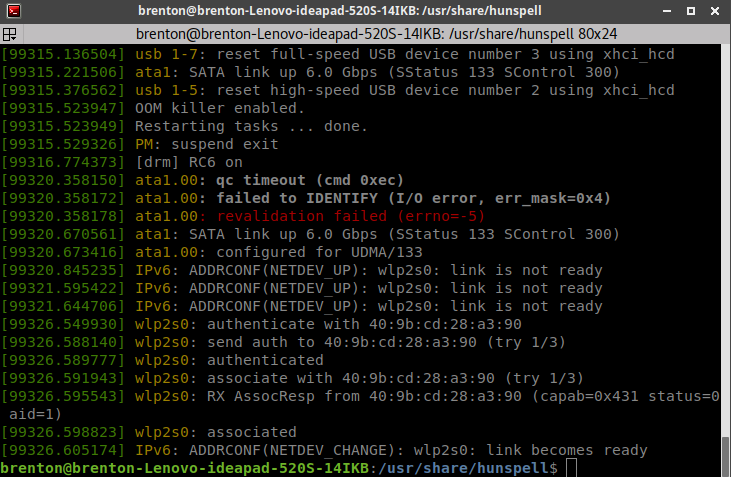
\includegraphics[scale=0.2]{test}
\end{figure}
\end{columns}
\end{frame}


\end{document}
